\documentclass[a4paper]{article}
%------ SETUP OF THE DOCUMENT ------%
%This part of the document sets up the document and makes it easier to read the main.tex file
%Changes in the setup file are recommended if you wish to customize things like colors in links and such.

%------ ********************* ------%
\usepackage[margin = 25mm]{geometry} %
\usepackage{graphicx} % Required for inserting images
\usepackage[toc,page]{appendix}
\usepackage[english=usenglishmax]{hyphsubst} %sets hyphenation to American English. Google is your friend on hyphenation. Babel could also be used
\usepackage[hyphens]{url}
\usepackage{amsmath, amssymb, setspace, float, subcaption, caption, booktabs, pdflscape, dcolumn, titlesec, tocloft, comment, xcolor, longtable, blindtext, rotating, lipsum}
\usepackage[flushleft]{threeparttable}
\usepackage[round, numbers, authoryear]{natbib}
\usepackage[hidelinks]{hyperref}
\usepackage{titlesec}
\usepackage{enumitem}

\hypersetup{
     colorlinks   = true, %If links to papers should be colored
     citecolor    = blue, %color of citation text
     urlcolor = blue, %if you use an URL, this is how it is colored
    linkcolor = black
}

\graphicspath{{figures/}}

%CHANGE SECTION STYLE

\bibliographystyle{apalike} %closest to LUSEM Harvard referencing guide

%%%%%%%%%%%%%%%%%%%%%%%%%%%%%%%%%%%
% Table formatting
%%%%%%%%%%%%%%%%%%%%%%%%%%%%%%%%%%%
\usepackage{multirow}


%%%%%%%%%%%%%%%%%%%%%%%%%%%%%%%%%%%
% Equation Formatting
%%%%%%%%%%%%%%%%%%%%%%%%%%%%%%%%%%%
\numberwithin{equation}{section}

%%%%%%%%%%%%%%%%%%%%%%%%%%%%%%%%%%%
% List Formatting
%%%%%%%%%%%%%%%%%%%%%%%%%%%%%%%%%%%
\setlist[itemize]{itemsep=0.05em}


\date{Seminar date}
\begin{document}

% TITLE PAGE 
\setstretch{1.5}

    %
\includegraphics[scale = 0.3]{images/LU RGB.png}
    %
\includegraphics[scale = 0.3]{images/LU Black.png} 
    
\includegraphics[scale = 0.15]{images/LUSEM_RGB.png} %I recommend using this one but the others are fine too
    %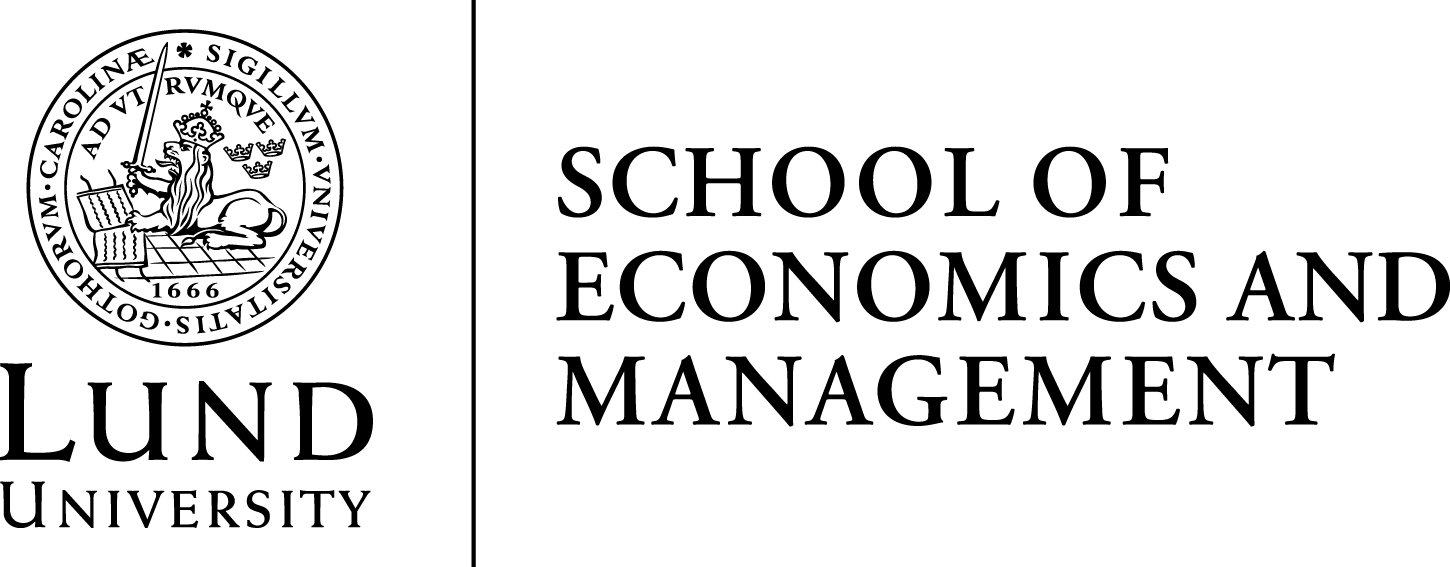
\includegraphics[scale = 0.15]{images/LUSEM_BLACK.png}

\vspace{2cm}
    \begin{center}       
        \vspace*{2cm}
        {\LARGE {\textbf{Means Testing in BAföG}  \\
        The Impact of Income Eligibility Thresholds on Student Labor Supply
        }} \\
        \vspace{1cm}
        \Large{María Sól Antonsdóttir \& Alexander Eriksson Byström} \normalsize{\\ Department of Economics \\ Lund University School of Economics and Management}
    \end{center}
    \vspace{2cm}

\vfill
\noindent 
\textbf{Supervisor: Petra Thiemann} \\ 
NEKN01 - Master Thesis in Economics 15 ECTS \\ 
Seminar date: Month Day, Year
\thispagestyle{empty}

\newpage
\tableofcontents
\thispagestyle{empty}


%%%%%%%%%%%%%%%%%%%%%%%%%%%%%%%%
% ABSTRACT
%%%%%%%%%%%%%%%%%%%%%%%%%%%%%%%%
\newpage
\begin{abstract}
\setstretch{1}
\lipsum[1] \\
    \noindent \textbf{Keywords:}  3 -- 5 key words\\
    \noindent \textbf{JEL codes:} Find appropriate codes at
    \url{https://www.aeaweb.org/econlit/jelCodes.php?view=jel}  %Standard in econ literature view=jel
\end{abstract}
\newpage
\setcounter{page}{1}

\hypersetup{linkcolor=blue}

%%%%%%%%%%%%%%%%%%%%%%%%%%%%%%%%
% CONTENT
%%%%%%%%%%%%%%%%%%%%%%%%%%%%%%%%
\section{Introduction} \label{sec:intro}
test \cite{xkcd}


%PREVIOUS LITERATURE
\section{LITERATURE} \label{sec:literature}

\section{Data}


\section{Method}


\subsection{Individual Students' Monthly Requirement}
The monthly requirement the student is eligible for is contingent on the financial support 
the student is currently receiving from his or her family. 
Firstly, the student receives a constant requirement of EUR 475, which is not contingent on the students' financial 
circumstances. To this basic amount the student receives requirements for \textbf{accommodation} (A), 
\textbf{health insurance} (HI), \textbf{long term care insurance} (LTCI) and an additional amount per the 
\textbf{number of children} (C) the student has. 
The requirement received for health insurance, long-term care insurance and accommodation is contingent on 
whether the parents are already providing these benefits. 
The total requirement the student will receive is therefore 

\begin{equation} \label{eq:total-requirement}
  \text{R} = 475 + \text{A} + \text{HI} + \text{LTCI} + \text{C}
\end{equation}
where
\begin{table}[H]
\small
\centering
  \begin{tabular}{lrr}
  \hline
  Variable & Provided by parents & Not provided by parents \\
  \hline
  A & 59 & 380 \\
  HI & 0 & 102 \\
  LTCI & 0 & 35 \\
  \hline
  \end{tabular}
\caption{Benefits contingent on parental provision (values in EUR).}
\end{table}







\subsection{Deductions from Requirement}
Parental and Student Income.

\begin{equation} \label{eq:parental-reduction}
  PR = \text{Parental Reduction} = 
  \begin{cases}
    0 & \text{if } E_5 \text{ or } (T_3 \text{ and } E_3) \\
    0 & \text{if } \text{Age}_{30} \\
    0.5 \times (\text{Parental Income} - \text{Exemption}) & \text{otherwise}
  \end{cases}
\end{equation}

\begin{itemize}
  \item \( E_5 \): Employed for 5 years after age 18
  \item \( T_3 \): Completed 3 years of vocational training
  \item \( E_3 \): Employed for 3 years after vocational training
  \item \( \text{Age}_{30} \): Older than 30 at the start of training
\end{itemize}

\begin{table}[H]
\small
\centering
  \begin{tabular}{lr}
  \hline
  Household Type & Exemption \\
  \hline
  Parents living together & 2,540 \\
  Parents live separately & 1,690 \\
  Spouse or Cohabiting Partner & 1,690 \\
  \hline
  \end{tabular}
\caption{Tax-free amount contingent on household type (values in EUR).} 
%NOTE: Add the fact that it's the penultimate year before approval period that is taken into consideration.
\end{table}

Let 
\[
SR = \text{Student Reduction} = 
\begin{cases} 
    0.5 \times \left( (\text{Income} - 556) + \max(0, \text{Assets} - 15,000)  \right) & \text{if Age}_{30} \\
    0.5 \times \left( (\text{Income} - 556) + \max(0, \text{Assets} - 45,000) \right) & \text{else}
\end{cases}
\]
\[
\text{BAföG}^\text{final}_{i} = \max(0, R - (PR + SR)) % Received BAföG amount
\]

% \[
% D_i = 
% \begin{cases}
% 1, & \text{if } \text{BAföG}_\text{final} = 0 \quad \text{(Ineligible for full requirement)} \\
% 0, & \text{otherwise}
% \end{cases}
% \]

Define a loss function out of the requirements and the deductions 
\begin{equation}
L(R, PR, SR) = R - (PR + SR)
\end{equation}


\subsection{Construction of Fuzzy RD}


Dummy variable for whether student loses any of his or her BAföG requirement
\begin{equation}
D_{i} = 
\begin{cases}
  1, \quad \text{if } L(R, PR, SR) > 0 \quad \text{(Some BAföG deduction occur)} \\
  0, \quad \text{if } L(R, PR, SR) = 0 \quad \text{(No deductions, full requirement)}
\end{cases}
\end{equation}

REVISE THIS ENTIRELY! Use a logit/probit for the first step then 
use these fitted values as regressor for second stage! 
Look into assumptions of both models and determine according to the 
characteristics of our data. 


First Stage (REVISE! Make into Logit/Probit)
\[ 
\text{BAFÖG}_{i} = \alpha + \beta D_{i} + \gamma X_{i} + \varepsilon_{i}
\]

Second Stage
\[ 
 \text{LabourSupply}_{i} = \delta + \lambda \widehat{\text{BAföG}}_{i} + \mu X_{i} + \nu_{i}
\]

\( \lambda \) coefficient for whether BAföG receipt reduces labour supply







%REFERENCES
\titleformat{\section}{\normalfont\huge\bfseries}{\thesection}{1em}{} 
\newpage
\addcontentsline{toc}{section}{References} 
\bibliography{bibliography}
\newpage

%APPENDICES
\appendix
\setcounter{page}{1} %Restarts page counting to 1
\pagenumbering{roman} %Differentiates the appendix page numbers from the main article

\titleformat{\section}{\centering\normalfont\normalsize\bfseries}{Appendix \thesection: }{0em}{}
\newpage
\section{Tables}
\renewcommand{\thetable}{\thesection \arabic{table}}
\setcounter{table}{0}


\begin{table}[H]
\centering
\renewcommand{\arraystretch}{0.8}  % Increase the height of the header
\begin{tabular}{lrrrr}
\hline
\hline
Year & \multicolumn{3}{c}{(\%) Supported Students} & Avg. Monthly Payment (2023 prices) \\
\cline{2-4}
     & Partially & Fully & Total & \\
\hline
1998 & 13 & 5 & 19 & 498.34 \\
1999 & 13 & 6 & 19 & 502.83 \\
2000 & 14 & 6 & 19 & 503.90 \\
2001 & 15 & 7 & 22 & 553.19 \\
2002 & 15 & 9 & 23 & 554.36 \\
2003 & 15 & 9 & 24 & 547.26 \\
2004 & 16 & 10 & 25 & 539.85 \\
2005 & 16 & 10 & 26 & 536.96 \\
2006 & 16 & 10 & 25 & 528.53 \\
2007 & 16 & 10 & 25 & 516.68 \\
2008 & 14 & 11 & 25 & 534.48 \\
2009 & 16 & 10 & 26 & 580.82 \\
2010 & 16 & 10 & 27 & 577.54 \\
2011 & 17 & 10 & 27 & 586.09 \\
2012 & 17 & 10 & 27 & 570.14 \\
2013 & 16 & 10 & 25 & 559.06 \\
2014 & 15 & 9 & 24 & 556.19 \\
2015 & 14 & 8 & 22 & 553.24 \\
2016 & 12 & 8 & 21 & 569.99 \\
2017 & 12 & 8 & 20 & 604.08 \\
2018 & 10 & 8 & 18 & 586.47 \\
2019 & 10 & 7 & 17 & 602.85 \\
2020 & 9 & 7 & 16 & 669.86 \\
2021 & 9 & 7 & 16 & 655.38 \\
2022 & 8 & 8 & 17 & 647.04 \\
2023 & 9 & 9 & 17 & 663.00 \\
\hline
\end{tabular}
\caption{
  Descriptives from 1998--2023 showing the fraction of HE students partially and fully 
  supported by BAföG, along with the average monthly payment adjusted for the German Consumer Price Index (CPI) from Destatis.
}
\label{tab:support_fraction_financial_expenditure}
\end{table}

\newpage
\section{Figures}
\renewcommand{\thefigure}{\thesection \arabic{figure}}
\setcounter{figure}{0}

\begin{figure}[H]
  \centering
  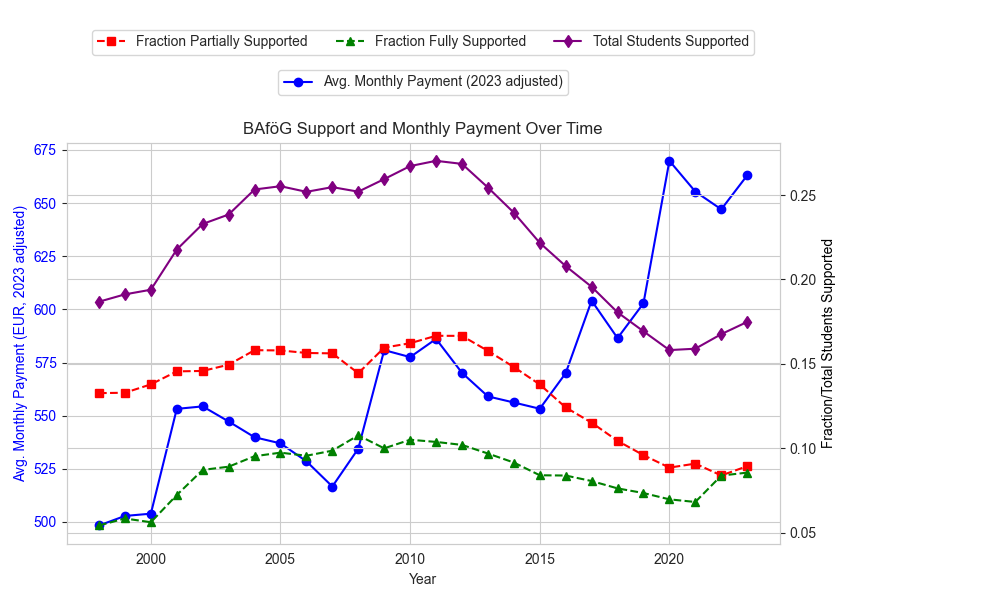
\includegraphics[width=0.95\linewidth]{bafog_support_over_time.png}
  \caption{
      Trends in CPI-adjusted average monthly payments from 1998 to 2023, expressed in 2023 prices. The figure also illustrates the fraction of enrolled students in Germany receiving partial, full, or combined partial and full loans and grants over the same period.
  }
  \label{fig:test}
\end{figure}

\end{document}
